% -- Encoding UTF-8 without BOM
% -- XeLaTeX => PDF (BIBER)

\documentclass[francais]{cv-style}          % Add 'print' as an option into the square bracket to remove colours from this template for printing. 
                                    % Add 'espanol' as an option into the square bracket to change the date format of the Last Updated Text

\sethyphenation{french}{PostgreSQL} % Add words between the {} to avoid them to be cut 
\exhyphenpenalty=10000
\hyphenpenalty=10000
\begin{document}

\header{Meili }{Vanegas-Hernandez} % Your name
\lastupdated

%----------------------------------------------------------------------------------------
%	SIDEBAR SECTION  -- In the aside, each new line forces a line break
%----------------------------------------------------------------------------------------

\begin{aside}
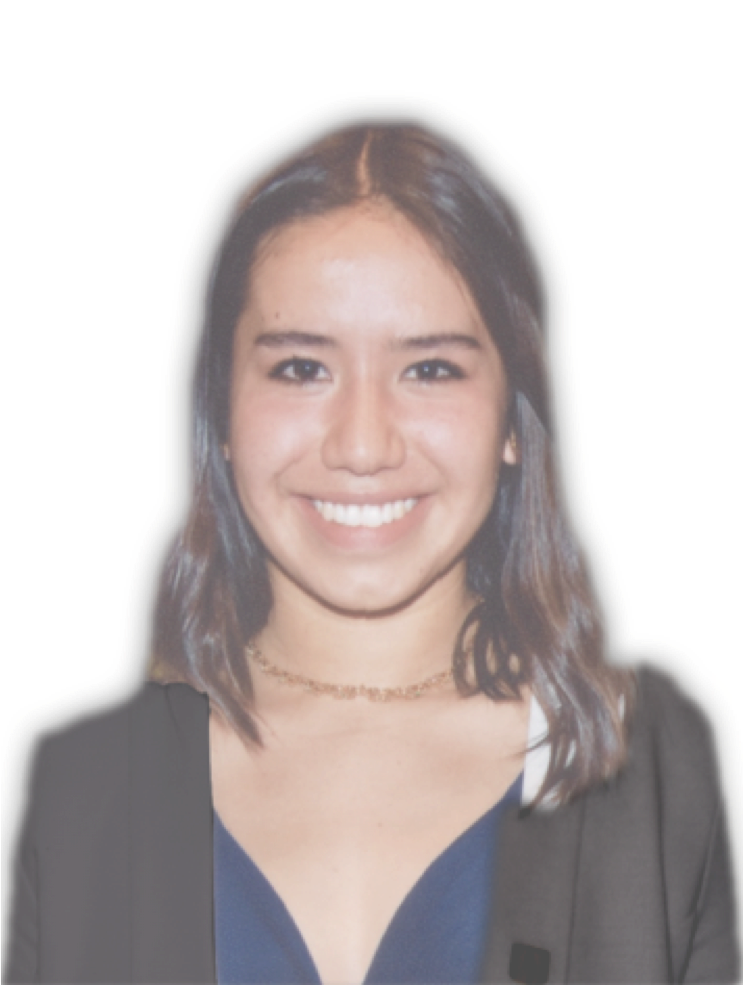
\includegraphics[width=3cm]{pictures/me.png}
%
\vspace{2.5cm}
\section{\textcolor{aquamarine}{contact}}\\
\vspace{0.2cm}
Bruxelles, Belgique\\
\vspace{0.1cm}
+32 (487) 71 55 87\\
\vspace{0.1cm}
{\href{mailto:meilivh8@gmail.com}{\underline{meilivh8@gmail.com}}}\\
\vspace{0.1cm}
{\href{https://mvanegas10.github.io}{\underline{https://mvanegas10.github.io}}}\\
%
\vspace{2.5cm}
\section{\textcolor{aquamarine}{langues}}\\
\vspace{0.2cm}
Espagnol (maternelle)\\
\vspace{0.1cm}
Anglais (expérimentée)\\
\vspace{0.1cm}
Français (avancée)\\
\vspace{0.1cm}
Allemand (élémentaire)\\
%
\vspace{2.5cm}
\section{\textcolor{aquamarine}{programming}}\\
\vspace{0.2cm}
{Python, JavaScript,\\
\vspace{0.1cm}
Java, C, SQL, Swift,\\
\vspace{0.1cm}
Matlab, \LaTeX{}, Visual\\
\vspace{0.1cm}
Basic, HTML, CSS}\\
\vspace{0.5cm}
{NodeJS, Jupyter\\
\vspace{0.1cm}
Notebooks, MongoDB,\\
\vspace{0.1cm}
Tableau, Django, D3.js,\\
\vspace{0.1cm}
AngularJS, ReactJS}\\
%
\end{aside}
%----------------------------------------------------------------------------------------
%	SKILLS SECTION
%----------------------------------------------------------------------------------------
\section{intérêts}
  \vspace{-0.2cm}
\textbf{professionnels :} analyse de données, visual analytics, mobilité et transport, urbanisme, big data, data science, machine learning, analyse et traitement des images, business intelligence. \textbf{personnels :} cyclisme, dessin, art, randonnée, photographie, natation, musique.

%----------------------------------------------------------------------------------------
%	WORK EXPERIENCE SECTION
%----------------------------------------------------------------------------------------

\section{expérience professionnelle }

\begin{entrylist}
%------------------------------------------------
\entry
  {02.2019\\}
  {STEER}
  {Bogota, Colombie}
  {\jobtitle{Consultante}\\
  Participation active dans le développement des modèles de transport pour les villes de Bogota et San Salvador.\\
  \bodyfontit{Création d'un outil visuel, permettant de comprendre les déplacements dans la matrice de voyages des grandes villes.}\\
    {\vspace{-0.1cm}}}
%------------------------------------------------
\entry
  {07.2017\\05.2018}
  {LABORATOIRE COMPUTER GRAPHICS \& HCI À TUK}
  {Kaiserslautern, Allemagne}
  {\jobtitle{Assistante de Recherche}\\
    Réalisation d'un outil d'analyse visuelle pour détecter les erreurs dans le processus de production dans une industrie. \\
    Projet de fin d'études : Développé avec des bioinformaticiens pour permettre l'identification et classification des séquences ADN et protéines.\\
    {\vspace{-0.1cm}}}
%------------------------------------------------
\entry
  {01.2017\\07.2017}
  {ALIANZA CAOBA}
  {Bogota, Colombie}
  {\jobtitle{Assistante de Recherche}\\
  Élaboration d’un projet de recherche en Big Data et analytique auprès du Ministère des Finances en Colombie afin d’identifier des fraudes ou évasions fiscales à Bogota. \\
    {\vspace{-0.1cm}}}
%------------------------------------------------
\entry
  {06.2016\\07.2016}
  {LABORATOIRE I3S ET ESPACE À L'UNIVERSITÉ SOPHIA ANTIPOLIS}
  {Nice, France}
  {\jobtitle{Chercheuse Junior }\\
  Stage en laboratoire d’urbanisme. Participation active dans l’élaboration du projet « Transport Oriented Modeling for Urban Densification Analysis » (TOMSA)/ECOS Nord. Réalisation d’un outil d’aide à la décision qui consiste en un modèle urbain à base d’agents (ABM) pour simuler les déménagements dans une ville sur un scénario spatial et évolutif. \\
    {\vspace{-0.1cm}}}
%------------------------------------------------


\end{entrylist}

%----------------------------------------------------------------------------------------
%	EDUCATION SECTION
%----------------------------------------------------------------------------------------

\section{formation}

\begin{entrylist}
%------------------------------------------------
\entry
{08.2017\\05.2018}
{M.Sc. {\normalfont Ingénierie Informatique}}
{Technische Universität Kaiserslautern}
{\bodyfontit{Concentration en Informatique Appliquée}\\
\normalfont{(ERASMUS)}\\
{\vspace{-0.1cm}}}
%------------------------------------------------
\entry
{01.2017\\05.2018}
{M.Sc. {\normalfont Ingénierie Informatique}}
{Université Los Andes}
{\bodyfontit{Concentration en Informatique Appliquée}\\
\normalfont{[4.30 (Échelle /5.0)]}\\
{\vspace{-0.1cm}}}
%------------------------------------------------
\entry
{08.2012\\12.2016}
{B.Sc. {\normalfont Ingénierie Informatique}}
{Université Los Andes}
{\normalfont{[4.08 (Échelle /5.0)]}\\
{\vspace{-0.1cm}}}
%------------------------------------------------
\entry
{07.2010\\05.2012}
{BI {\normalfont Programme du diplôme}}
{Gimnasio Vermont}
{\normalfont{[27 Points]} \\
{\vspace{-0.5cm}}}
%------------------------------------------------
\end{entrylist}

%----------------------------------------------------------------------------------------
%	OTHER QUALIFICATIONS SECTION
%----------------------------------------------------------------------------------------

\section{projets et concours}

\begin{entrylist}
%------------------------------------------------
\entry
{2016\\\vspace{-0.3cm}}
{Hackathon Cognitiva (Premier Prix)}
{IBM, UniAndes, Alianza Caoba}
{\vspace{-0.3cm}}
%------------------------------------------------
\entry
{2015\\\vspace{-0.3cm}}
{Concours Innovation des TI (Deuxième Prix)}
{Université Los Andes}
{\vspace{-0.3cm}}
%------------------------------------------------
\entry
{2012\\\vspace{-0.5cm}}
{Summa Cum Laude}
{Gimnasio Vermont}
{\vspace{-0.5cm}}
%------------------------------------------------
\end{entrylist}

\end{document}